\documentclass[12pt,english]{article}
\usepackage[a4paper,bindingoffset=0.2in,%
            left=1in,right=1in,top=1in,bottom=1in,%
            footskip=.25in]{geometry}
\usepackage{blindtext}
\usepackage{titling}
\usepackage{amssymb}
\usepackage{amsmath}
\usepackage{listings}
\usepackage{lettrine} 
\usepackage{tikz}  
\usepackage{color} 
\usepackage{verbatim}
\usepackage{pgfplots}
\usepgfplotslibrary{external}
\pgfplotsset{width=10cm,compat=1.9}
%================================
\begin{document}
\newgeometry{left=0.8in,right=0.8in,top=1in,bottom=1in}
\begin{center}
    \Large
    \textbf{Homework 7}\\
    \small
    \today\\
    \large
    Jose Carlos Munoz
\end{center}%===============================
Q6.a)\\
Q6.b)\\
Q6.c)\\
Q6.d)\\
Q6.e)\\
Q16)\par
The Following is for the Single Link\\
This is the similarity matrix from each of the points.
\begin{equation*}
\begin{array}{c|ccccc}
\mbox{-}& 1 & 2 & 3 & 4 & 5\\
\hline
1 & 1.00 & 0.10 & 0.41 & 0.55 & 0.35 \\
2 & 0.10 & 1.00 & 0.64 & 0.47 & 0.98 \\
3 & 0.41 & 0.64 & 1.00 & 0.44 & 0.85 \\
4 & 0.55 & 0.47 & 0.44 & 1.00 & 0.76 \\
5 & 0.35 & 0.98 & 0.85 & 0.76 & 1.00 
\end{array}
\end{equation*}\\
From this set we can see that the value with the highest similarity is 2 and 5, so they are cluster together to form cluster 2,5\\
\begin{equation*}
\begin{array}{c|ccccc}
\mbox{-}& 1 & 2 & 3 & 4 & 5\\
\hline
1 & 1.00 & 0.35 & 0.41 & 0.55 & 0.35 \\
2 & 0.35 & 1.00 & 0.85 & 0.76 & 1.00 \\
3 & 0.41 & 0.85 & 1.00 & 0.44 & 0.85 \\
4 & 0.55 & 0.76 & 0.44 & 1.00 & 0.76 \\
5 & 0.35 & 1.00 & 0.85 & 0.76 & 1.00 
\end{array}
\end{equation*}
From this set we can see that the value with the highest similarity is cluster 2,5 and 3, so they are cluster together to form cluster 2,5,3\\
\begin{equation*}
\begin{array}{c|ccccc}
\mbox{-}& 1 & 2 & 3 & 4 & 5\\
\hline
1 & 1.00 & 0.41 & 0.41 & 0.55 & 0.41 \\
2 & 0.41 & 1.00 & 1.00 & 0.76 & 1.00 \\
3 & 0.41 & 1.00 & 1.00 & 0.76 & 1.00 \\
4 & 0.55 & 0.76 & 0.44 & 1.00 & 0.76 \\
5 & 0.41 & 1.00 & 1.00 & 0.76 & 1.00 
\end{array}
\end{equation*}
From this set we can see that the value with the highest similarity is cluster 2,5,3 and 4, so they are cluster together to form cluster 2,5,3,4\\
\begin{equation*}
\begin{array}{c|ccccc}
\mbox{-}& 1 & 2 & 3 & 4 & 5\\
\hline
1 & 1.00 & 0.55 & 0.55 & 0.55 & 0.55 \\
2 & 0.55 & 1.00 & 1.00 & 1.00 & 1.00 \\
3 & 0.55 & 1.00 & 1.00 & 1.00 & 1.00 \\
4 & 0.55 & 1.00 & 1.00 & 1.00 & 1.00 \\
5 & 0.55 & 1.00 & 1.00 & 1.00 & 1.00 
\end{array}
\end{equation*}
From this set we can see that the value with the highest similarity is cluster 2,5,3,4 and 1, so they are cluster together to form cluster 2,5,3,4,1\\
Now we display the graph made from these clusters.
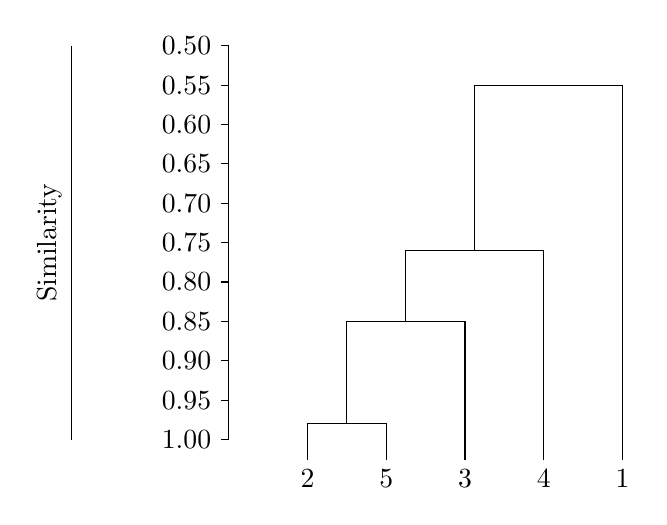
\begin{tikzpicture}[sloped]
    \node (a) at (-6,-0.5) {2};
    \node (b) at (-5,-0.5) {5};
    \node (c) at (-4,-0.5) {3};
    \node (d) at (-3,-0.5) {4};
    \node (e) at (-2,-0.5) {1};
    \node (ab) at (-5.5,0.2) {};
    \node (abc) at (-4.75,1.5){};
    \node (abcd) at (-3.875,2.4) {};
    \node (abcde) at (-2.9375,4.5) {};
    
    \draw  (a) |- (ab.center);
    \draw  (b) |- (ab.center);
    \draw  (c) |- (abc.center);
    \draw  (d) |- (abcd.center);
    \draw  (e) |- (abcde.center);
    \draw  (ab.center) |- (abc.center);
    \draw  (abc.center) |-(abcd.center);
    \draw  (abcd.center) |-(abcde.center);
 
    \draw[] (-9,0) -- node[above]{Similarity} (-9,5);
    \draw (-7,0) -- (-7,5);
    
    \foreach \y in {0,0.5,1,1.5,2,2.5,3,3.5,4,4.5,5}                     
    \draw[shift={(0,\y)},color=black] (-7,0) -- (-7.1,0);
    
    \node[left] at (-7.1,0.0) {$1.00$} ;
    \node[left] at (-7.1,0.5) {$0.95$} ;
    \node[left] at (-7.1,1.0) {$0.90$} ;
    \node[left] at (-7.1,1.5) {$0.85$} ;
    \node[left] at (-7.1,2.0) {$0.80$} ;
    \node[left] at (-7.1,2.5) {$0.75$} ;
    \node[left] at (-7.1,3.0) {$0.70$} ;
    \node[left] at (-7.1,3.5) {$0.65$} ;
    \node[left] at (-7.1,4.0) {$0.60$} ;
    \node[left] at (-7.1,4.5) {$0.55$} ;
    \node[left] at (-7.1,5.0) {$0.50$} ;
    
\end{tikzpicture}
\par
The Following is for the Complete Link\\
This is the similarity matrix from each of the points.
\begin{equation*}
\begin{array}{c|ccccc}
\mbox{-}& 1 & 2 & 3 & 4 & 5\\
\hline
1 & 1.00 & 0.10 & 0.41 & 0.55 & 0.35 \\
2 & 0.10 & 1.00 & 0.64 & 0.47 & 0.98 \\
3 & 0.41 & 0.64 & 1.00 & 0.44 & 0.85 \\
4 & 0.55 & 0.47 & 0.44 & 1.00 & 0.76 \\
5 & 0.35 & 0.98 & 0.85 & 0.76 & 1.00 
\end{array}
\end{equation*}
From this set we can see that the value with the highest similarity is 2 and 5, so they are cluster together to form cluster 2,5\\
\begin{equation*}
\begin{array}{c|ccccc}
\mbox{-}& 1 & 2 & 3 & 4 & 5\\
\hline
1 & 1.00 & 0.10 & 0.41 & 0.55 & 0.10 \\
2 & 0.10 & 1.00 & 0.64 & 0.47 & 1.00 \\
3 & 0.41 & 0.64 & 1.00 & 0.44 & 0.64 \\
4 & 0.55 & 0.47 & 0.44 & 1.00 & 0.47 \\
5 & 0.10 & 1.00 & 0.64 & 0.47 & 1.00 
\end{array}
\end{equation*}
From this set we can see that the value with the highest similarity is cluster 2,5 and 3, so they are cluster together to form cluster 2,5,3\\
\begin{equation*}
\begin{array}{c|ccccc}
\mbox{-}& 1 & 2 & 3 & 4 & 5\\
\hline
1 & 1.00 & 0.10 & 0.10 & 0.55 & 0.10 \\
2 & 0.10 & 1.00 & 1.00 & 0.44 & 1.00 \\
3 & 0.10 & 1.00 & 1.00 & 0.44 & 1.00 \\
4 & 0.55 & 0.44 & 0.44 & 1.00 & 0.44 \\
5 & 0.10 & 1.00 & 1.00 & 0.44 & 1.00 
\end{array}
\end{equation*}
From this set we can see that the value with the highest similarity is cluster 1 and 4, so they are cluster together to form cluster 1,4\\
\begin{equation*}
\begin{array}{c|ccccc}
\mbox{-}& 1 & 2 & 3 & 4 & 5\\
\hline
1 & 1.00 & 0.10 & 0.10 & 1.00 & 0.10 \\
2 & 0.10 & 1.00 & 1.00 & 0.10 & 1.00 \\
3 & 0.10 & 1.00 & 1.00 & 0.10 & 1.00 \\
4 & 1.00 & 0.10 & 0.10 & 1.00 & 0.10 \\
5 & 0.10 & 1.00 & 1.00 & 0.10 & 1.00 
\end{array}
\end{equation*}
From this set we can see that the value with the highest similarity is cluster 2,5,3 and 1,4 so they are cluster together to form cluster 2,5,3,4,1\\
Now we display the graph made from these clusters.
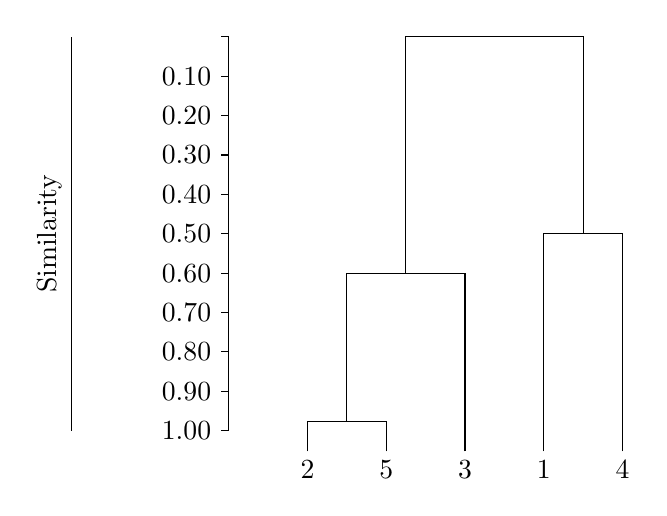
\begin{tikzpicture}[sloped]
    \node (a) at (-6,-0.5) {2};
    \node (b) at (-5,-0.5) {5};
    \node (c) at (-4,-0.5) {3};
    \node (d) at (-3,-0.5) {1};
    \node (e) at (-2,-0.5) {4};
    \node (ab) at (-5.5,0.11) {};
    \node (abc) at (-4.75,2){};
    \node (cd) at (-2.5,2.5) {};
    \node (abcde) at (-2.9375,5) {};
    
    \draw  (a) |- (ab.center);
    \draw  (b) |- (ab.center);
    \draw  (c) |- (abc.center);
    \draw  (d) |- (cd.center);
    \draw  (e) |- (cd.center);
    \draw  (ab.center) |- (abc.center);
    \draw  (abc.center) |-(abcde.center);
    \draw  (cd.center) |-(abcde.center);
 
    \draw[] (-9,0) -- node[above]{Similarity} (-9,5);
    \draw (-7,0) -- (-7,5);
    
    \foreach \y in {0,0.5,1,1.5,2,2.5,3,3.5,4,4.5,5}                     
    \draw[shift={(0,\y)},color=black] (-7,0) -- (-7.1,0);
    
    \node[left] at (-7.1,0.0) {$1.00$} ;
    \node[left] at (-7.1,0.5) {$0.90$} ;
    \node[left] at (-7.1,1.0) {$0.80$} ;
    \node[left] at (-7.1,1.5) {$0.70$} ;
    \node[left] at (-7.1,2.0) {$0.60$} ;
    \node[left] at (-7.1,2.5) {$0.50$} ;
    \node[left] at (-7.1,3.0) {$0.40$} ;
    \node[left] at (-7.1,3.5) {$0.30$} ;
    \node[left] at (-7.1,4.0) {$0.20$} ;
    \node[left] at (-7.1,4.5) {$0.10$} ;
    
\end{tikzpicture}
\par
Q17.a)\\
Q17.b)\\
Q17.c)\\
Q17.d)\\
Q17.e)\\
Q17.f)\\
\end{document}
